\section{Introduction}
\label{sec:introduction}
3D printers have the basic task of extruding filament at a given x, y, z
coordinate at time t. The mechanism that achieves that movement
determines the machine's costs, print quality, and robustness. Out of
many different options, the Core XY mechanism is a popular choice
for modern printers. Unlike Cartesian designs, where one
motor drives one axis, here each motor simultaneously changes the
x and y position of the tool head (see Figure~\ref{fig:printer_schematic}).
This results in a more complex kinematic model, but allows a sturdier
casing and faster printing speeds. Our task is to model and simulate the system.

\begin{figure}[htbp]
  \centering
  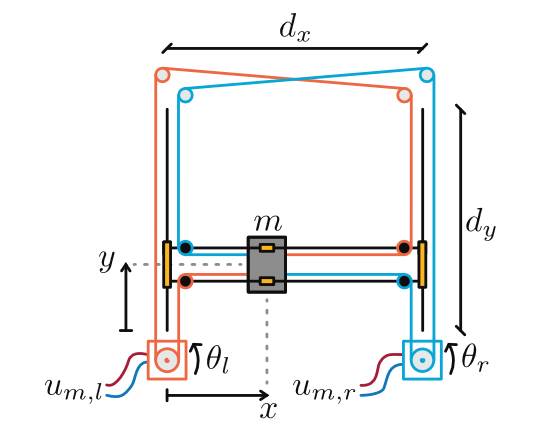
\includegraphics[width=0.6\textwidth]{printer_sch.png}
  \caption{Schematic of the Core XY mechanism.}
  \label{fig:printer_schematic}
\end{figure}

\subsection{Symbol Table}
\label{sec:symbol_table}

%% Table generated by Claude, but I found the hidden values :)
% also I changed the rotational friction to be in Nms / rad, because I already modeled it as a rotational friction
\begin{table}[H]
  \centering
  \caption{Symbols and parameter values.}
  \label{tab:symbols}
  \begin{tabular}{llr}
    \toprule
    Description & Symbol & Value \\
    \midrule
    Motor angle left                  & $\theta_L$      & -- \\
    Motor voltage left                & $u_{m,L}$       & -- \\
    Motor current left                & $i_L$           & -- \\
    Motor radius                      & $r_m$           & \qty{11}{\milli\metre} \\
    Motor inductance                  & $L_m$           & \qty{10}{\milli\henry} \\
    Motor resistance                  & $R_m$           & \qty{90}{\ohm} \\
    Motor inertia                     & $J_m$           & \qty{8e-6}{\kilogram\metre\squared} \\
    Motor constant                    & $K_m$           & \qty{0.07}{\newton\metre\per\ampere} \\
    \midrule
    Tool head position                & $x$, $y$        & -- \\
    Tool head mass                    & $m$             & \qty{60}{\gram} \\
    \midrule
    Nozzle voltage                    & $u_n$           & -- \\
    Nozzle inductor current           & $i_{L,n}$       & -- \\
    Nozzle capacitance                & $C_n$           & -- \\
    Nozzle inductance                 & $L_n$           & -- \\
    Capacitor voltage                 & $u_c$           & -- \\
    Nozzle thermal capacity           & $C_{t,n}$       & -- \\
    Nozzle thermal resistance         & $R_{t,n}$       & \qty{9}{\kelvin\per\watt} \\
    Nozzle resistance                 & $R_n$           & \qty{8}{\ohm} \\
    Resistor thermal capacity         & $C_r$           & -- \\
    Resistor temperature              & $T_r$           & -- \\
    Thermal resistance to environment & $R_{\mathrm{env}}$ & -- \\
    Reference resistance              & $R_0$           & -- \\
    Reference temperature             & $T_0$           & -- \\
    Temperature coefficient of resistance & $\alpha$    & -- \\
    Nozzle temperature                & $T_n$           & \qty{240}{\degreeCelsius} \\
    Environmental temperature         & $T_e$           & \qty{26.85}{\degreeCelsius} \\
    \midrule
    Bearing friction rolling          & $\mu_r$         & \qty{2.7e-8}{\newton\metre\second\per\radian} \\
    Bearing friction linear $x$-direction & $\mu_{l,x}$ & \qty{0.002}{\newton\second\per\metre} \\
    Bearing friction linear $y$-direction & $\mu_{l,y}$ & \qty{0.001}{\newton\second\per\metre} \\
    Bearing radius                        & $r_b$       & \qty{3}{\milli\metre} \\
    \midrule
    Print bed temperature             & $T_b$           & \qty{105}{\degreeCelsius} \\
    Print area dimension $x$          & $d_x$           & \qty{29}{\centi\metre} \\
    Print area dimension $y$          & $d_y$           & \qty{29}{\centi\metre} \\
    \bottomrule
  \end{tabular}
\end{table}
